\documentclass[conference]{IEEEtran}
\usepackage[cmex10]{amsmath}
\usepackage{xcolor}
\usepackage{graphicx}
\hyphenation{op-tical net-works semi-conduc-tor}

\begin{document}
\title{Week 4 Report\\ECE 432 Microwave Circuit Design II}
\author{\IEEEauthorblockN{Jackson Pugh}
\IEEEauthorblockA{Portland State University\\
Portland, OR 97207\\
Email: japugh@pdx.edu}
\and
\IEEEauthorblockN{Michael Woodruff}
\IEEEauthorblockA{Portland State University\\
Portland, OR 97207\\
Email: michael.woodruff@pdx.edu}}
\maketitle
\IEEEpeerreviewmaketitle
\section{Introduction}
Goal of this session is to explore simulation tools (ADS) usage in design for stability, noise and gain. We will use SAV-541+ transistor and you should have its S2P parameters stored somewhere that’s easily accessible. We will follow the first 30 pages or so from reference\cite{payne}. Basic idea is to apply the same techniques explained in there but to our own transistor. For our overall FSK receiver project your design has to cover 2.4 – 2.6 GHz range with at least 10dB of gain. Noise figure should be minimized but it is not of primary importance, i.e. it can be sacrificed for gain.
\section{Questions \& Answers}
1. Design a bias network for SAV-541+ transistor with VDS=3V and IDS=60 mA. Present schematic and result for your design. You can use any of the several designs in various application notes but you may want to start with a simple resistive design.\\\\
a. Investigate and comment on sensitivity of your bias to variations of component values.\\
b. Comment on how well your design will “integrate” with future matching network that you will design (i.e. think about this as you design your bias circuit).\\\\
\textcolor{red}{Figure~\ref{fig:dccircuit} shows the DC bias network for the SAV-541+ transistor.  It was determined from the SAV-541+ I-V curves that the gate voltage applied to the MOSFET transistor needed to be 0.5 V ($V_{GS}$) to obtain a 60 mA $I_{DS}$ current, thus the resistor divider was chosen to give a close match (however, some additional tweaking was required to get the current closer).   The BJT current mirror also acts to bias/force $I{DS}$ to be 60 mA.  The supply power was chosen to be 3.7 V (instead of 3.3 V) due to the 0.7 V drop from the BJT current mirror.  An additional resistor was required (R6) to produce the 3 V drain to source voltage.  Figure~\ref{fig:dcvalues} shows the screenshot result from the DC simulation in ADS.  The results from the bias network are accurate.  There are several critical components that determine the biasing of the transistor.  These include the voltage divider at the gate and the resistor that determines the current being drawn at the current mirror.}

\begin{figure}[!h]
\centering
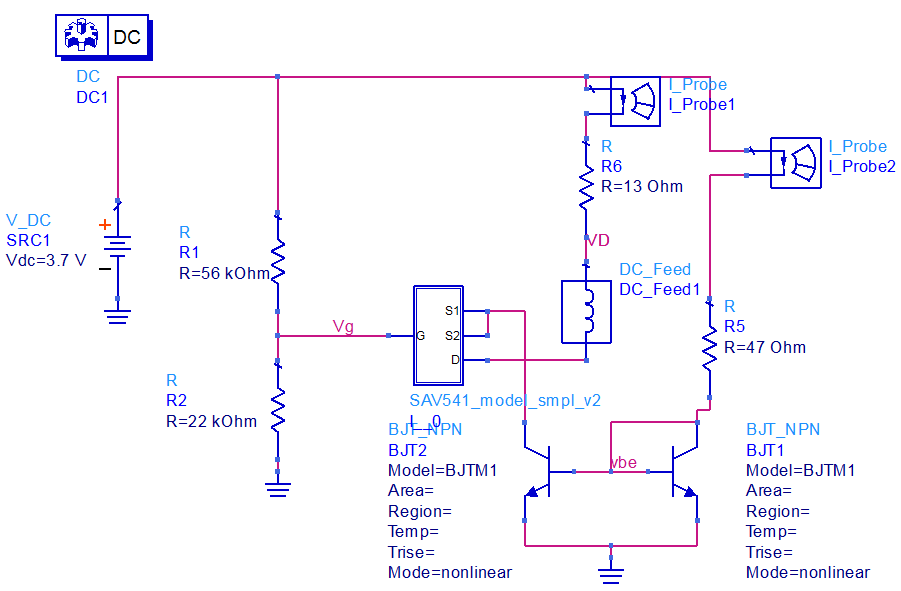
\includegraphics[scale=0.35]{pics/dcbiascircuit.png}
\caption{DC bias network for the SAV-541+ transistor.}
\label{fig:dccircuit}
\end{figure}
\begin{figure}[!h]
\centering
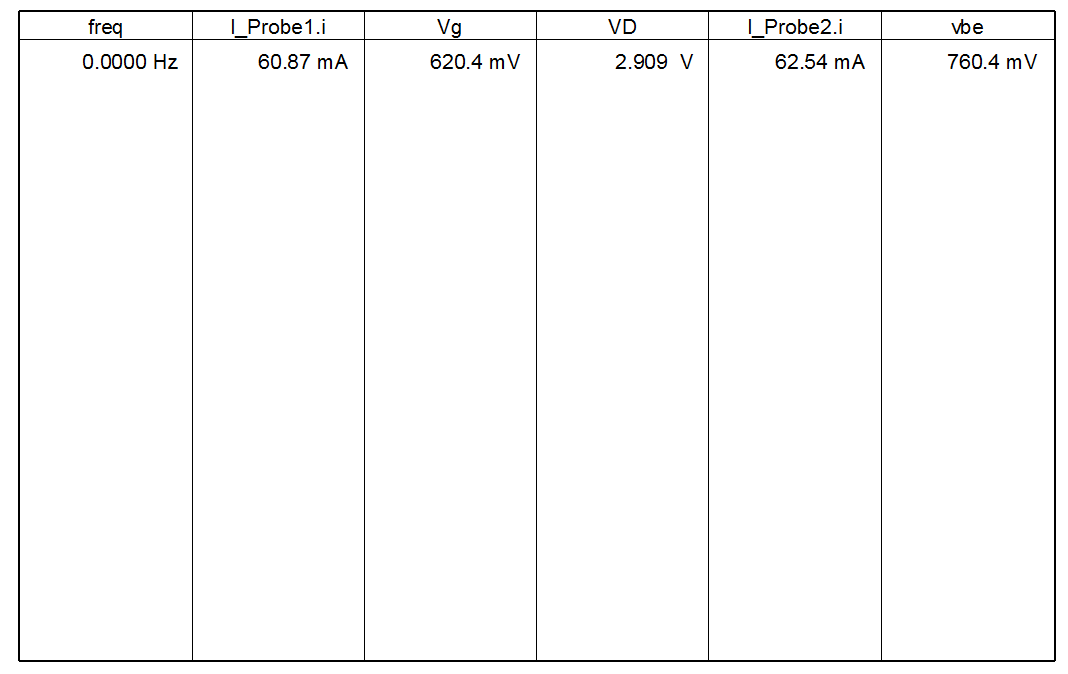
\includegraphics[scale=0.31]{pics/biasvalues.png}
\caption{Current and voltage  parameters from the DC bias network for the SAV-541+ transistor.}
\label{fig:dcvalues}
\end{figure}
2. Do a "quick" comparison between S-parameters given by the manufacturer and S-parameters you get from a model that was distributed. Report back if you find any significant discrepancies, in particular in $|$S21$|$.\\\\
\textcolor{red}{Figure~\ref{fig:sparamcircuit} shows the S-Parameter biased network transistor circuit.  Figure~\ref{fig:sparamresult} shows the S-Parameters comparison between the untuned bias network circuit and the manufacturer S2P data.  The bias network shows little discrepency.}

\begin{figure}[!h]
\centering
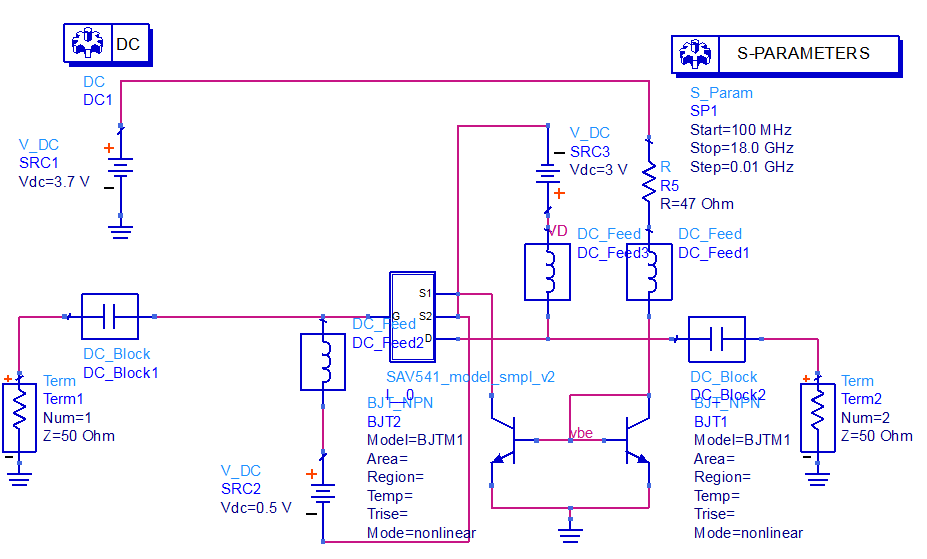
\includegraphics[scale=0.35]{pics/sparametercomparison-circuit-untuned.png}
\caption{S-Parameter bias network for the SAV-541+ transistor.}
\label{fig:sparamcircuit}
\end{figure}
\begin{figure}[!h]
\centering
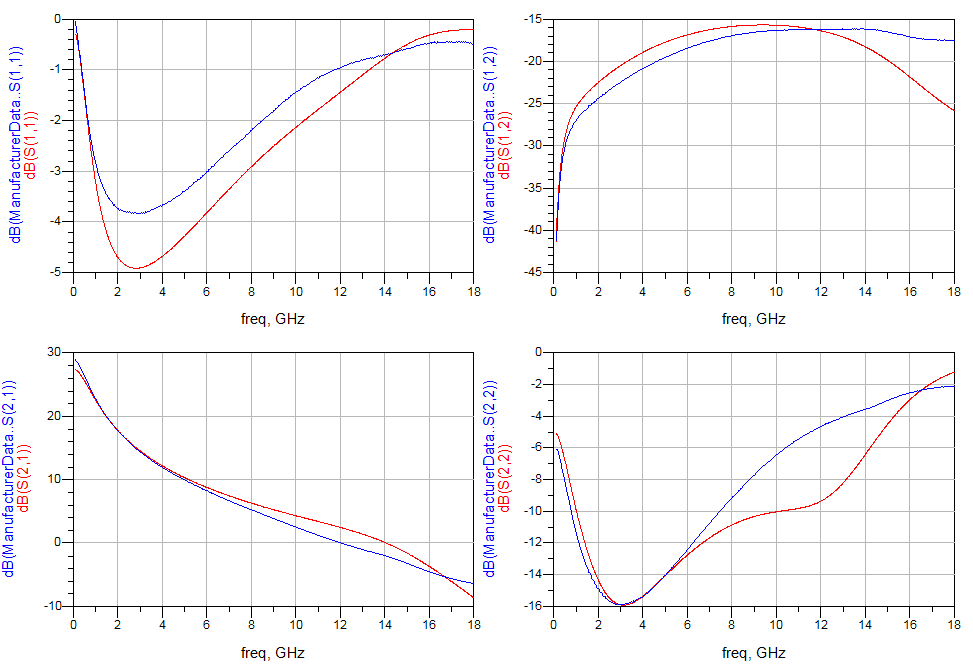
\includegraphics[scale=0.35]{pics/sparametercomparison-untuned.png}
\caption{S-Parameter simulation result comparison between the bias network and the manufacturer S2P data file.}
\label{fig:sparamresult}
\end{figure}
3. Using ADS design guide for amplifiers, reproduce figure 13 from\cite{payne}. In your report comment on the amount of gain and stability. Limit your frequency range to 0.1 – 6 GHz. Do you anticipate any problems based on these results?\\\\
\textcolor{red}{Figure~\ref{fig:designguide} shows various information provided by the ADS amplifier design guide tool.  The circuit is potentially unstable below around 4 GHz.  Thus, stabilizing resistors will be necessary in order to make the transistor unconditionally stable between 2.4 - 2.6 GHz (the intended frequency range).}

\begin{figure}[!h]
\centering
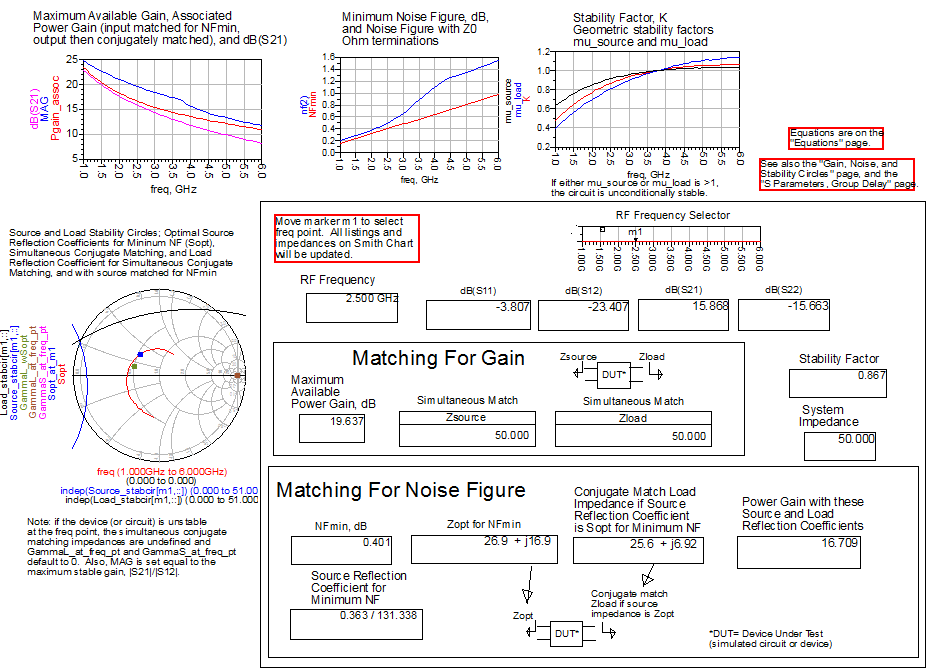
\includegraphics[scale=0.35]{pics/designguide.png}
\caption{Amplifier design guide generated in ADS for the bias network for the SAV-541+ transistor.}
\label{fig:designguide}
\end{figure}
%4. Decide on circuit that you will use to stabilize your transistor and make appropriate changes in DesignGuide, as explained in [1]. Examine your results carefully – just because simulation is converging (or appears to be converging!) does not mean that the results make sense. Once you are satisfied with your design, include schematic (Figure 14) and results (Fig 15). If possible, use “standard” component values or, even better, components that are available in IEEE store.
%5. Add SMD component models from the library and see if parasitic effects change your results – see pages 18 – 21 in [1]. Re-optimize your stability circuit, as needed.
%6. Add ground inductance into source lead of SAV 541+. Start with 0.4 nH and increase it to 1 nH. What effect does it have on noise, gain and stability?
%7. Design a “final” stabilizing circuit that will ensure stability across 0.1 – 6 GHz range and satisfy the criteria for gain and NF in our LNA project.
%8. Final step involves designing either for maximum gain or some smaller value. Now that you have unconditionally stable device you can do simultaneous conjugate match. What gain do you simulations predict?
%9. This may have to be done after the lab session: integrate your bias and matching networks and produce a layout. For SAV-541+ we don’t have a built-in footprint so you will have to replace it with some other “dummy” device that uses the same package (one option may be Avago Technologies ATF-34143 that Payne uses). Remember what you learned from your previous project with respect to placement of SMD components and effects of even small length of transmission line that appears in signal path. Make sure that you include DC blocking capacitor on input and output.

%\newpage
%\section{Weekly Lessons}
%\subsection{In-Class}
%\subsection{Outside of Class}
\begin{thebibliography}{1}
\bibitem{payne}
K. Payne, "Practical RF Amplifier Design Using the Available Gain Procedure and the Advanced Design System EM/Circuit Co-Simulation Capability," Agilent Technologies (5990-3356EN), 2008.
\end{thebibliography}
\end{document}